\chapter{Instabilità e riconnessione}

\begin{teorema}{di connessione (conservazione del flusso)}{}
	
	\begin{multicols}{2}
	Per capire cosa vuol dire che le linee di campo non si rompono e perché, prendiamo due elementi di fluido infinitamente vicini, $d\vec l$, dopo un tempo dt ciascun punto si muove con la velocità del fluido, $\vec x \rightarrow \vec x + \vec u(\vec x)dt$. 
	\begin{figure}[H]
		\centering
		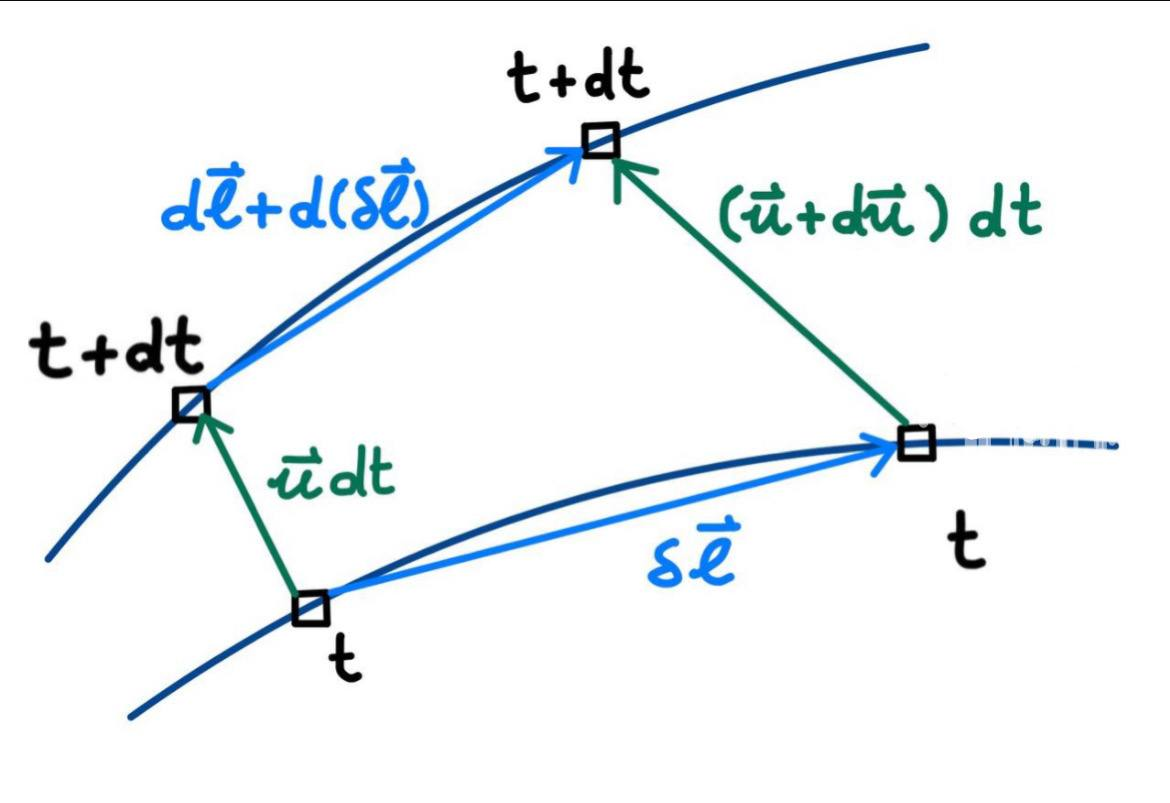
\includegraphics[width=5cm]{immagini/flusso3.jpg}
	\end{figure}
	
	\end{multicols}
	
	\[d\vec l+d(\delta\vec l)=d\vec l+ \left[ (\vec u+d\vec u)-\vec u \right] dt \ =\ d\vec l+d\vec udt
	\implies
	d(\delta\vec l)=d\vec udt\]  
	
	$d\vec u$ è l'incremento del campo di velicità in direzione $d\vec l$
	
	\[d\vec u=(d\vec l\cdot \vec \nabla)\vec u\] 
	
	\[d\vec l+\delta (d\vec l)=d\vec l+ \left[ \vec u(\vec x+d\vec x)-\vec u (\vec x)\right] dt \ =\ d\vec l+(d\vec l\cdot \nabla)\, \vec u\, dt \] 
	
	Capiamo quindi che la variazione nel tempo della distanza fra i due elementi che si muovono è descritto da $\frac{d(\delta\vec l)}{dt}=(\delta \vec l\cdot\vec \nabla)\vec u$. Nota che se $d\vec l$ è lungo una linea di campo allora $d\vec l \times \vec B = 0$, noi ci chiediamo se partendo solo dalle equazioni dell'elettromagnetismo possiamo provare che queste linee di campo non si spezzino.
	Quindi vogliamo calcolare: 
	
	\[\frac{d}{dt}(\delta\vec l\times\vec B)\ =\ \frac{d\delta\vec l}{dt}\times \vec B\,+\,\delta\vec l\times\frac{d\vec B}{dt}\]
	
	Consideriamo la legge di faraday e la legge di Ohm ideale:
	
	\[ \frac{\partial\vec B}{\partial t}\ =\ -\nabla \times \vec E
	\quad \qquad \quad 
	\vec E\ =\ -\,\frac{\vec u \times \vec B}{c} \]
	
	\[\Rightarrow\qquad \frac{\partial\vec B}{\partial t}\ =\ \vec \nabla\times(\vec u\times\vec B)\]
	
	Seguiamo $\vec B$ attraverso una linea di campo facendo la derivata materiale, questo ci servirà subito l'evoluzione delle linee di campo. Per semplificare l'espressione ci ricordiamo (insomma)  un'identità vettoriale:
	
	\[\frac{D\vec B}{Dt}=\frac{\partial\vec B}{\partial t}+(\vec u\cdot \vec \nabla)\cdot \vec B=(*)\]
	
	\[\vec \nabla\times(\vec u\times\vec B)\ =\ \vec u\,\cancel{( \vec \nabla \cdot \vec B)}-\vec B( \vec \nabla \cdot\vec u) + (\vec B \cdot \vec\nabla)\,\vec u-(\vec u\cdot\vec \nabla)\cdot \vec B\]
	
	\[(*)=\ \vec \nabla\times(\vec u\times\vec B) + (\vec u\cdot \vec \nabla) \vec B\ =\ (\vec B\cdot \vec \nabla)\, \vec u - \vec B\, (\vec \nabla\cdot \vec u)\] 
	
	Sostituendo $\partial\vec B/\partial t$ con l'identità vettoriale, il termine con gradiente della derivata materiale si elide e possiamo cancellare anche  $\vec \nabla\cdot \vec B=0$ per via della seconda equazione di Maxwell.
	
	Allora inserendo questo risultato di $\partial\vec B/\partial t$ assieme a quello prima definito già definito all'inizio di $\frac{d(\delta\vec l)}{dt}=(\delta \vec l\cdot\vec \nabla)\vec u$, si trova infine che l'evoluzione della connesione fra i due elementi fluidi segue: 
	
	\[\frac{d}{dt}(\delta\vec l\times\vec B)=\delta\vec l\times \left[(\vec B\cdot\vec \nabla )\vec u+(\vec B\cdot\vec \nabla )\vec u\right]  +(\delta\vec l\cdot\vec\nabla)\vec u\times\vec B\] 
	
	\vspace{0.5cm}
	
	Se si considera il caso $\delta \vec l\parallel\vec B$, che implica $\delta \vec l\times \vec B = 0$, allora  $\delta\vec l\times(\vec B\cdot\vec \nabla) \vec u=0$ e la formula trovata poco fa va ad annullarsi completamente portando a $\frac{D}{Dt}(\delta \vec l \times \vec B)=0$: per vederlo basta porre $\delta\vec l$ come un riscalamento $\alpha \vec B$:
	
	
	\[\boxed{\frac{d}{dt}(\delta\vec l\times\vec B)=\alpha\vec B\times \left[\cancel{(\vec B\cdot\vec \nabla )\vec u}+(\vec B\cdot\vec \nabla )\vec u\right]  +(\alpha \vec B \cdot\vec\nabla)\vec u\times\vec B \ =\ \dots\ =\ 0}\] 
	
	Si vede abbastanza già così come si annulli tutto grazie alla condizione di parallelismo.
	
	Questo risultato ci porta a osservare che la linea di campo non si rompe finché non avviene la \textit{riconnessione}. Per  violare la legge di Ohm devo avere $\eta\vec J$, sono questi i casi in cui può avvenire la riconnessione (la legge dio Ohm viene violata prima alle scale degli ioni e poi dopo viene violata alle scale degli elettroni).
	
	\[S=\frac{T_r}{T_a}=\frac{T_\text{resistivo}}{T_\text{alfvén}}\] 
	
	La resistività fa capire come in tempi molto più brevi del tempo diffusivo cambia la topologia del campo. 
	
	Flusso magnetico: su una superficie chiusa fa zero, in generale è 
	\[\int_S\vec B\cdot d\vec S\ =\ \Phi (\vec B)\] 
\end{teorema}

\begin{teorema}{Alfvén}{}
	Finché siamo in MHD ideale vale che:
	\[ \boxed{\ \frac{d\Phi (\vec B)}{dt}\ =\ 0\ }\]  
	
	\begin{multicols}{2}
		\begin{figure}[H]
			\centering
			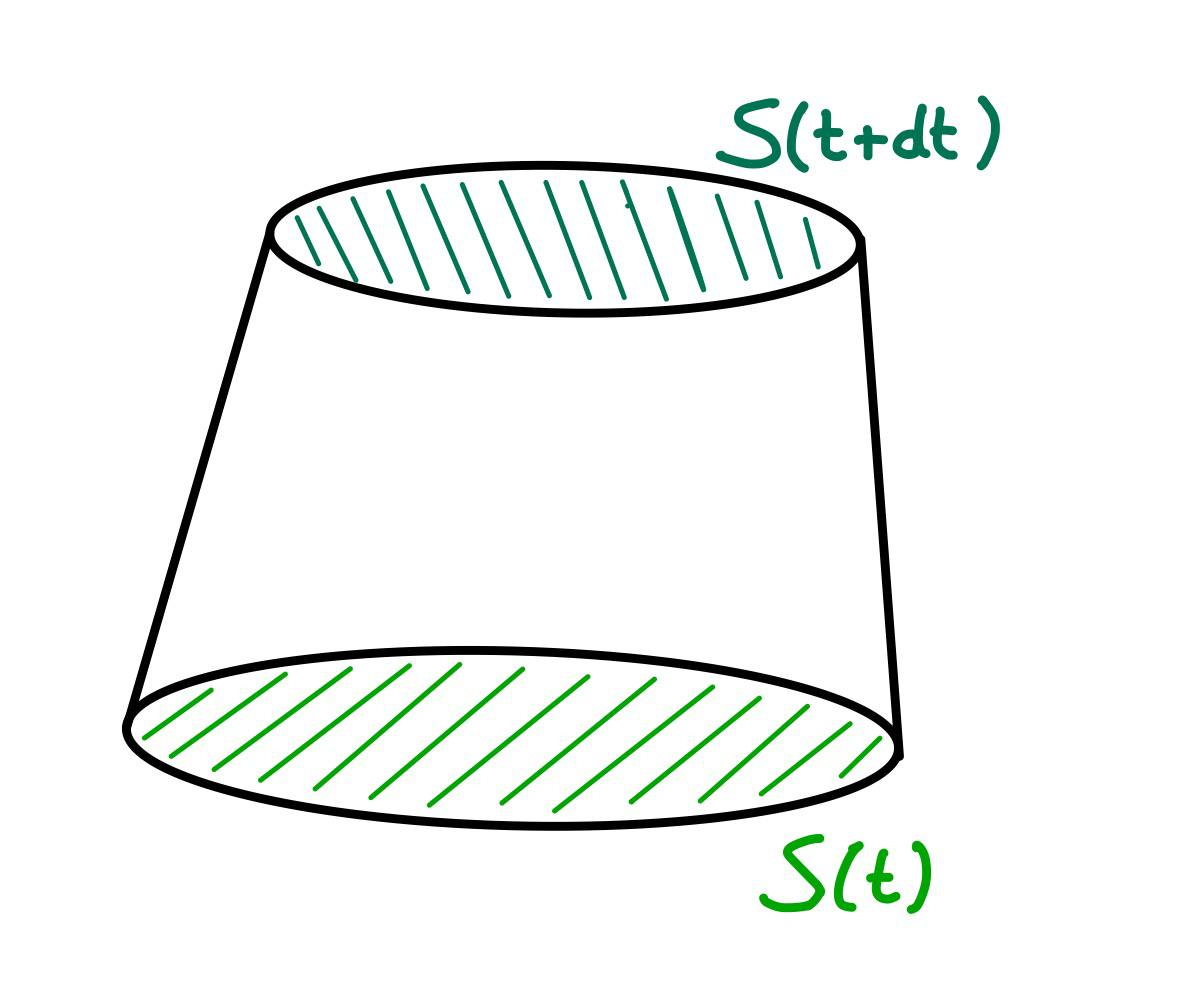
\includegraphics[width=4cm]{immagini/flusso1.jpg}
		\end{figure}
		
		\begin{figure}[H]
			\centering
			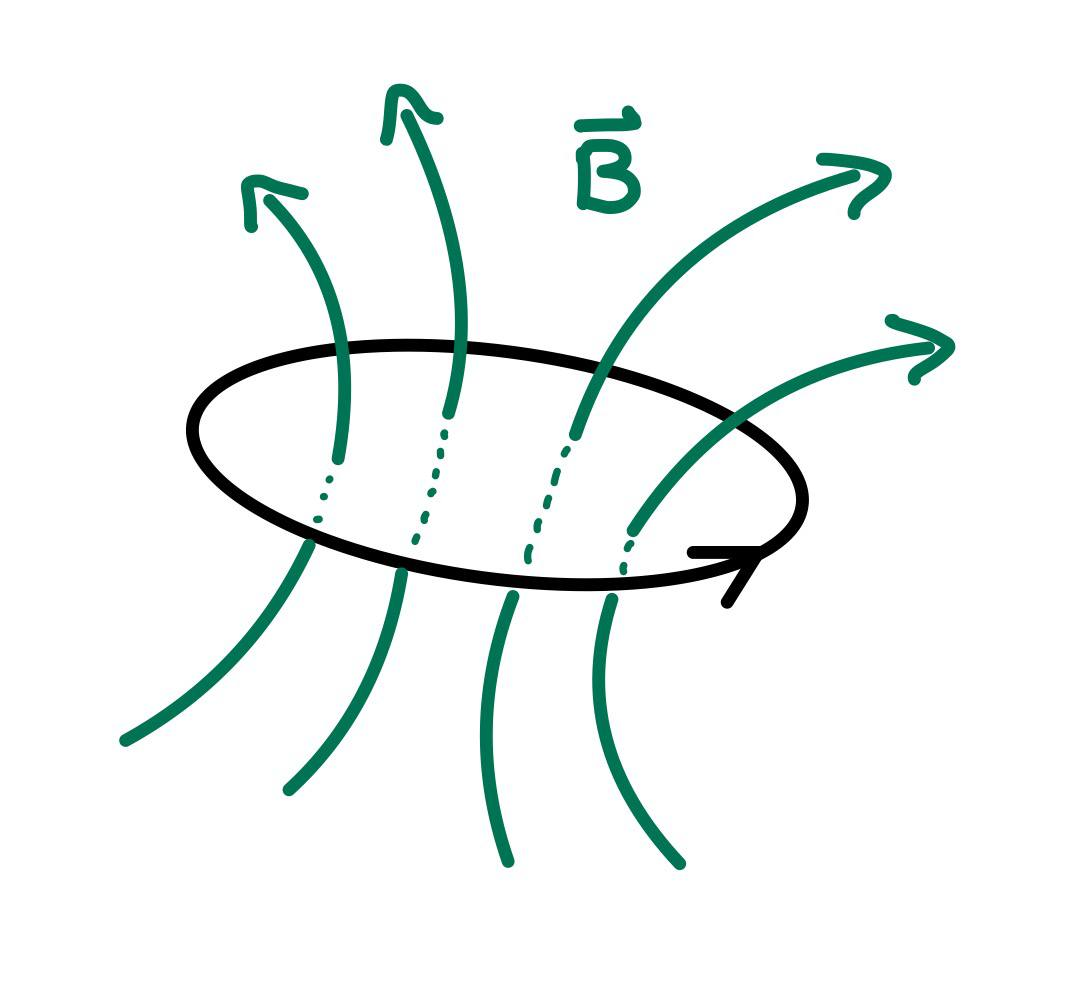
\includegraphics[width=4cm]{immagini/flusso2.jpg}
		\end{figure}
	\end{multicols}
	
	Usando il teorema di Leibnitz per integrare su domini mobili scomponiamo la derivata del flusso in un primo termine, variazione locale di flusso dovuta al cambiamento di B nel tempo, ed un secondo termine invece rappresenta il cambiamento dovuto al fatto che $\mathcal{C}$ :
	
	\[\frac{d}{dt}\int_{S(t)}\vec B(\vec r,t)\cdot d\vec S
	\ =\
	\int_{S(t)}\frac{\partial \vec B}{\partial t}\cdot d\vec S+\oint_{\mathcal{C}(t)}\vec B\cdot (\vec u\times d\vec l)\] 
	
	Il primo termine del termine al membro destro è la variazione locale di flusso dovuta al cambiamento di B nel tempo, il secondo termine invece rappresenta il cambiamento dovuto al fatto che $\mathcal{C}$ si è mosso: 
	
	Usiamo il fatto che $\vec B\cdot (\vec u\times d\vec l)=-\vec u\times \vec B\cdot d\vec l$ ed il teorema di Stokes.
	
	\[\frac{d\Phi}{dt}
	\ =\
	\frac{d}{dt}\int_{S(t)}\vec B(\vec r,t)\cdot d\vec S
	\ =\
	\int_{S(t)}\bigg(\frac{\partial}{\partial t}\vec B-\nabla\times(\vec u\times \vec B)\bigg)d\vec S\]  
	
	in MHD ideale è valida la legge di Ohm ideale $\frac{\partial\vec B}{\partial t}=\vec \nabla\times(\vec u\times\vec B)$ e quindi 
	
	\[\frac{\partial}{\partial t}\vec B-\nabla\times(\vec u\times \vec B)\ =\ 0
	\ \implies\ 
	\int_{S(t)}\bigg(\frac{\partial}{\partial t}\vec B-\nabla\times(\vec u\times \vec B)\bigg)d\vec S\ =\ 0\]  
	
	ed abbiamo così dimostrato il teorema per cui $\boxed{\frac{d\Phi}{dt} = 0}$ .
\end{teorema}


%
\section{Instabilità di Kelvin-Helmholtz}

\begin{figure}[H]
	\centering
	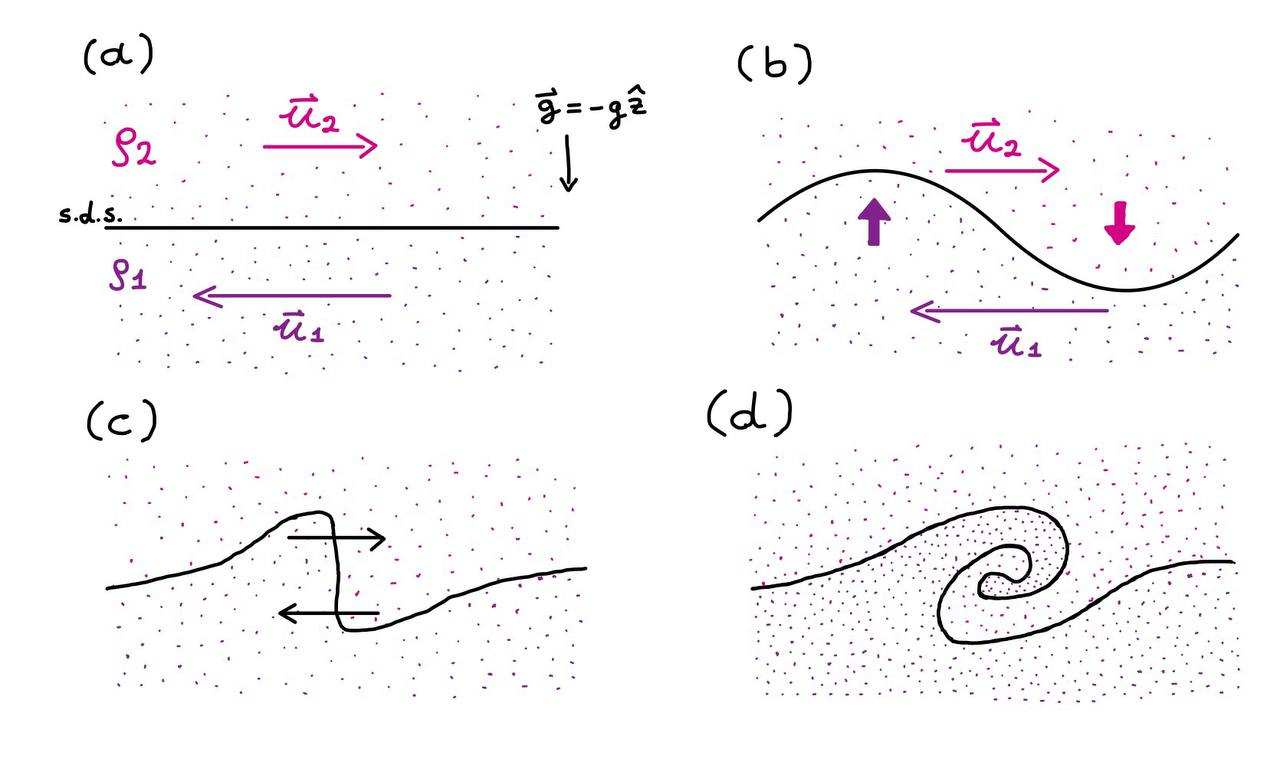
\includegraphics[width=0.8\linewidth]{immagini/KH.jpg}
\end{figure}

\[\begin{cases}
	\vec \nabla \cdot \vec u\ =\ 0\\
	\rho_0 \frac{\partial \vec v}{\partial t}\, +\, (\vec v\cdot \vec \nabla )\, \vec v\ =\ -\nabla P\, +\, \rho_0 \vec g
\end{cases}\]

Prendiamo il rotore dell'equazione con $\vec \nabla \times \vec v = \vec \omega$

\[ \rho_0 \frac{\partial \vec v}{\partial t}\, +\, \nabla \left(\frac{v^2}{2}\right) - \vec v \times \vec \omega\ =\ 0\]

\[ \rho_0 \frac{\partial \vec \omega}{\partial t}\ =\ \vec \nabla\times \left(\vec v\times \vec \omega\right) \]

Prendiamo solo la parte solenoidale di $\vec v$ mentre la parte rotazionale non contribuisce $\iff \vec v =\vec \nabla \phi \iff \vec \omega = 0$.

Cerchiamo le soluzioni dell'equazione imponendo $\vec v = \vec \nabla \phi$:

\[\phi\ =\ \begin{cases} \phi_1\ ,\quad z<0\\ \phi_2\ ,\quad z>0 \end{cases}\]

Parametrizzando la superficie di scorrimento come $\xi (x,y,t)$ e consideranzo che per $z\to \pm \infty$ la velocità $\vec u\to 0$

\[\vec u_2\ =\ \frac{D \xi}{D t}\ =\ \frac{\partial \xi}{\partial t} + \frac{\partial \xi}{\partial x}\frac{\partial x}{\partial t} + \cancelto{\text{secondo ordine}}{\frac{\partial \xi}{\partial y}\frac{\partial y}{\partial t}}\]

Ora facendo i calcoli che si farebbero per l'instabilità di Kelvin-Helmholtz in fluidodinamica si giunge a:

\[
\gamma\ =\ -\frac{im(\rho_1 u_1+\rho_2 u_2)}{\rho_1 + \rho_2}\, \pm \, \left[m^2\rho_1 \rho_2\frac{(u_1 - u_2)^2}{(\rho_1 + \rho_2)^2}\, -\, ky\frac{\rho_1 - \rho_2}{\rho_1 + \rho_2}\right]^{1/2}
\]

Vediamo due casi particolari:
\begin{itemize}
	\item Se $\rho_1=\rho_2=\rho$ si ha un K-H "puro":
	\[ \gamma\ =\ -\,i\,m\, \frac{u_1 + u_2}{2}\, \pm \, m\left[ \frac{(u_1 - u_2)^2}{4} \right]^{1/2} \]
	\item Se $u_1 = u_2 = u$:	
	\[\gamma\ =\ i\, \left[mu\, \pm\, \left( k y\frac{\rho_1 - \rho_2}{\rho_1 + \rho_2}\right)^{1/2}\right]\]
\end{itemize}





%%
%
%
\section{Riconnessione} 
La riconnessione è una transizione verso uno stato di energia minore che sarebbe proibita per la MHD ideale, ma può accadere in MHD resistiva, venendo violata localmente la legge di OHM ideale in una regione  (detta zona ad x  o zona resistiva) di dimensione caratteristica $\delta$  infinitesima rispetto al sistema totale, permettendo così una rottura delle linee di campo.

Viene cambiata globalmente la topologia  creando una cosidetta isola di campo, inoltre viene liberata una grandissima quantità di energia Questa quantità di energia viene presa dalla struttura stessa del campo che si riarrangia nella sua interezza in una configurazione meno energetica.

Matematicamente abbiamo un'eq differenziale al quart'ordine "struttura tipo \underline{strato limite} in fluidodinamica" (fidati). 

Il termine del quart'ordine $\boxed{\eta\frac{d^4}{dx^4}\bar b}$ non conta mai tranne che nelle regioni di grandi gradienti perché è guidato da un coefficiente piccolissimo, d'altra parte è proprio questo termine invece a guidare la soluzione nelle regioni interne (zona ad x) dove si hanno forti gradienti in cui $\displaystyle\frac{d}{dx}\sim\frac{1}{\delta}$ e $\delta$ è la lunghezza caratteristica dello strato resistivo,  che va raccordata alla soluzione delle regioni esterne in cui invece $\frac{d}{dx}\sim\frac{1}{L}$.

$L$ è la dimensione caratteristica MHD "lunghezza scala del campo di equilibrio". 

Stiamo lavorando in una regione in cui la relazione fra tempo caratteristico \underline{resistivo} e \underline{di Alfvén} consiste in $\tau_A\,\ll\, 1/\gamma\,\ll\,\tau_R$, con $\gamma$ che è la stessa in $f(x)\, exp(i k y\pm \gamma t)$ in modo da poter definire:

\[1\ \ll\ \frac{1}{\gamma\tau_a}\ \ll\ \frac{\tau_A}{\tau_R}\ \equiv\  S\ \equiv\ R_a\quad \text{che è un numero enorme}\] 

Noi osserviamo chiaramente che la riconnessione avviene anche in 3D ma per il momento la studiamo in 2D.

\subsubsection{Riconnessione in 2D:}

Le condizioni del problema sono che ci mettiamo in 2D ($\partial_z=0$) in approssimazione incomprimibile $\vec\nabla\cdot\vec u=0$ e: 

\[\vec B=B_0(x)\hat y+\vec b\hspace{1cm}u_z\,=\,0=\,b_z\ ,\hspace{1cm} \vec u_0=0\]


Praticamente l'intensità del campo magnetico seguendo l'asse x ha valori asintotici $B_0$ per $x\to\infty$ e $-B_0$ per $x\to-\infty$. poi c'è una zona di alto gradiente di dimensioni caratteristiche L lunghezza scala del campo di equilibrio, 

\[L\sim\frac{B_0}{B_0'} \hspace{1cm}L\gg\delta\]

Per fare un esempio dell'andamento tipico possiamo considerare  $B_0(x)=\tanh{\frac{x}{L}}$ 

I campi di variazione sono 

\[\vec b=b_x(x,y)\hat x+b_y(x,y)\hat y,\hspace{1cm}\vec u=u_x(x,y)\hat x+u_y(x,y)\hat y\] 

Dalla fluidodinamica sappiamo che possiamo scrivere il campo 2D come gradiente di un campo ausiliario

\[\vec b=\nabla\psi\times\hat z=\partial_y\psi\hat x-\partial_x\psi\hat y,\hspace{1cm}\vec u=\nabla\phi\times\hat z=\partial_y\phi\hat x-\partial_x\phi\hat y\] 

Dopodiché ho bisogno dell'equazione di Faraday ("dell'induzione") 


%
%
%
\subsection{equazione di faraday}  Vorrei tanto sapere come mai l'equazione di faraday è proprio scritta così, io non me la ricordo mica come siarriva a questo punto e mi auguro di scoprirlo presto... cmq davanti ad eta potrebbe esserci un $4\pi$ o comunque una costante

\[\partial_t\, \vec B\ =\ \nabla\times(\vec u\times\vec B_0)\ +\ \eta\,\nabla^2\vec b\]

facciamo tutti i conti passo passo
\[\vec u\times\vec B_0= 
\begin{vmatrix} 
	\hat i & \hat j & \hat k\\ 
	\partial_y\phi & \partial_x\phi & 0\\
	0& B_0 &  0
\end{vmatrix} 
=B_0\partial_y\phi\hat z\] 

\[\nabla\times[\vec u\times\vec B_0]= 
\begin{vmatrix} 
	\hat i & \hat j & \hat k\\ 
	\partial_x & \partial_y & 0\\
	0& 0 &  B_0\partial_y\phi
\end{vmatrix} 
\ =\ B_0\partial_{yy}\phi\hat x-\partial_x[B_0\partial \phi]\hat y\ =\ B_0\partial_{yy}\phi\hat x-(B_0'\partial_y\phi+B_0\partial_{xy}\phi)\hat y\] 

dove $B_0'=\partial_ xB_0$ e in generale d'ora in poi i termini col primo si intende derivata lungo x. 

\[\nabla^2\vec b\ =\ (\partial_{xx}+\partial_{yy})(\partial_y\psi\hat e_x-\partial_x\psi\hat e_y)\ =\ (\partial_{xxy}+\partial_{yyy})\psi\hat e_x\,-\,(\partial_{xxx}+\partial_{yyx})\psi\hat e_y\] 

chiaramente la derivata rispetto al tempo del campo elettrico mi ammazza il campo medio $B_0$ 

\[\partial_t\vec B=\partial _t\vec b=\partial_{ty}\psi\hat x-\partial_{tx}\psi\hat e_y\]

Metto tutto insieme , separo le componenti e impongo una soluzione piana $\sim f(x)e^{iky-\gamma t}$.

\begin{itemize}
	\item componente $\hat e_x$:\[ \partial_{ty}\psi\ =\ B_0\partial_{yy}\phi\,+\,\eta\,(\partial_{xxy}+\partial_{yyy})\psi\] tutti i termini contengono un $\partial _y$ e quindi posso integrare in $\partial y$.\\
	\[\gamma\psi\ =\ ikB_0\phi\,+\,\eta(\psi''-k^2\psi)\] 
	\item componente y:  \\ho ricucito la derivata del prodotto. 
	\[ -\partial_{tx}\psi\ =\ -(B_0\partial_y\phi)'\,-\,\eta(\partial_{xxx}-\partial_{yyx})\psi\]
	
\end{itemize} 

Infine mi interesso di normalizzare l'equazione praticamente in temini di $L,\tilde c_a, \tilde B$ che sono i valori caratteristici di $\phi$ e di $\psi$. compare il termine  parente stretto di $\eta$, $\frac{t_a}{t_r}=S^{-1}$.  
alla fine dela fiera quello che viene fuori è per quanto riguarda la componente x  
\[\gamma\psi=ikB_0\phi+S^{-1}(\psi''-k^2\psi)\] Attenzione !!! e la componente y quanto fa??

%
%
\subsection{equazione del moto } dall'incomprimibilità si ha sicuramente che non vi sono variazioni nella densità che è uniformemente $\rho_0$.;\\ il termine $\vec u\nabla\cdot\vec u$ è del second'ordine e lo lasciamo perdere sin da subito.  
\[ \rho_0\partial_t(\nabla\times\vec u)=\frac{1}{4\pi}\nabla\times[(\nabla\times \vec B)\times\vec B]\]
intanto sicuramernte posso linearizzare e mi trovo solamente i termini di primo grado. 
\[ \rho_0\partial_t(\nabla\times\vec u)=\frac{1}{4\pi}\nabla\times[(\nabla\times \vec b)\times\vec B_0]+\frac{1}{4\pi}\nabla\times[(\nabla\times \vec B_0)\times\vec b]\] 
ora di nuovo bisogna fare  i prodotti vettoriali e i rotori per benino benissimo
\[\nabla\times \vec b=\begin{vmatrix}
	\hat i&\hat j&\hat k\\
	\partial x &\partial_y& 0\\
	\partial_y\psi&-\partial _x\psi&0
\end{vmatrix}=-(\partial_{xx}\psi+\partial_{yy}\psi)\hat z\] 
\[\nabla\times\vec u=-(\partial_{xx}\phi+\partial_{yy}\phi)\hat z\]
\[\nabla\times \vec B_0=\begin{vmatrix}
	\hat i&\hat j&\hat k\\
	\partial x &\partial_y& 0\\
	0&B_0&0
\end{vmatrix}=\partial _x B_0\hat z=B_0'\hat z\] \[(\nabla\times\vec b)\times\vec B_0=
\begin{vmatrix}
	\hat i&\hat j&\hat k\\
	0 & 0& -(\partial_{xx}+\partial_{yy})\psi\\
	0 & B_0& 0
\end{vmatrix}=B_0(\partial_{xx}+\partial_{yy})\psi\hat x \]
\[(\nabla\times\vec B_0)\times\vec b=
\begin{vmatrix}
	\hat i&\hat j&\hat k\\
	0&0&B'_0\\
	\partial_y\psi&\partial_x\psi&0
\end{vmatrix}
=B_0'\partial_x\psi\hat x+B_0'\partial_y\psi\hat y\] 

\[\nabla\times[(\nabla\times \vec b)\times\vec B_0]=
\begin{vmatrix}
	\hat i& \hat j&\hat k \\
	\partial _x&\partial_y&0\\
	B_0(\partial_{xx}+\partial_{yy})\psi&0&0
\end{vmatrix}
=-B_0(\partial_{yxx}+\partial_{yyy})\psi\hat z\] 
\[\nabla\times[(\nabla\times \vec B_0)\times\vec b]
=
\begin{vmatrix}
	\hat i& \hat j&\hat k \\
	\partial _x&\partial_y&0\\
	B_0'\partial_x\psi&B_0'\partial_y\psi&0
\end{vmatrix}
=[\partial_x(B_0'\partial_y\psi)-B_0'\partial_{yx}\psi]\hat z=\]\[=[B_0''\partial_y\psi+B_0'\partial_{yx}\psi-B_0'\partial_{yx}\psi]\hat z=B_0''\partial_y\psi\hat z\]

\[4\pi\rho_0\partial_t(\partial_{xx}+\partial_{yy})\phi=B_0(\partial_{yxx}+\partial_{yyy})\psi-B_0''\psi\] imponendo una soluzione di tipo onda piana (oddio non è mica vero che è un'onda piana... chiedere) le derivate rispetto al tempo fanno scendere un $\gamma$, le derivate seconde rispetto ad x danno un doppio primo, le derivate seconde rispetto a y danno $-k^2$.  ora bisogna normalizzare e $\gamma$ lo normalizzo col tempo di alfven, $\phi $ è una velocità  per una lunghezza e quindi va diviso per $\tilde c_aL$, se moltiplico per $L^2$ normalizzo sia la derivata seconda rispetto a x sia rispetto a $k^2$. 
\[\frac{\tau_aL^2}{L\tilde c_a}=\frac{L^2}{\tilde c_a L/\tau_a}\sim\frac{L^2}{\tilde c_a^2}\] allora se moltiplico il membro a sx per $\tau_a\frac{L}{\tilde c_a}$ mi rimane la densità $\rho_0$. dall'altra parte la $\psi$ è $\sim \tilde BL\implies \psi''$ e anche $k^2\psi\sim \frac{\tilde B}{L}$ contando anche il $k$ davanti a tutto e il campo magnetico hoche il membro a dx è $\sim B^2/L^2$. il fattore con cui ho moltiplicato il membro a sx mi fa diventare il membro a destra $\sim \frac{\tilde B}{\tilde c_a^2}$.\\Se riesco a capire che $\rho_0\sim\frac{\tilde B^2}{c_a^2}$ sono a cavallo. \\in alternativa mi piace anche magari che $\rho_0\sim\frac{\tilde B}{c_a^2}$  perché comunque mi va bene che sia in termini del campo magnetico.  
\\Credo che ho bisogno dell'equazione di continuità per riuscire a dimensionare campo magnetico e densità. 

%
%
\subsection{equazioni MHD incomprimibile} 
\begin{enumerate}
	\item \[\gamma(\phi''-k^2\phi)=ikB_0(\psi''-k^2\psi)-ikB_0\psi\]
	\item \[\gamma\psi-ikB_0\phi=S^{-1}(\psi''-k^2\psi)\] è da qui che emerge l'equazione differenziale del uart'ordine. il termine alla derivata quarta è effettivamente quello legato al numero di Raynolds magnetico, $S^{-1}$ è un numero piccolissimo e sono necessari grandi gradienti per farlo uscire fuori. Queste equazioni presentano una singolarità ed è in quel punto che comincia a contare il termine del quart'ordine. Quando la velocità di fase dell'onda di alfven matcha la velocità del suono locale ovvero quando $\frac{\omega}{k}\sim c_a(x_0)$ in $x_0$ c'è la singolrità. Avere questa singolarità non necessariamente porta ad una riconnessione, è infatti questo il caso anche per le oscillazioni di kelvinhelmoltz  in cui le onde fanno risonanza con la disomogeneità e dissipano l'energia, però se il campo magnetico passa da zero e fa un'inversione "si inverte", posso avere la riconnsessone. in questo caso l'energia  viene liberata dal campo medio che cambiando configurazione passa ad uno stato di minore energia. \\
	
	DOMANDA:
	
	Ma nel caso di KelvinHelmoltz avviene un cambiamento di Topologia?  
\end{enumerate}

%
%
\subsection{ipotesi e time ordering}  
\begin{itemize}
	\item H1: assumo che esistano due regioni con diversi regimi \begin{itemize}
		\item REGIONE IDEALE \\ in cui il termine resistivo non conta e in questa zona i gradienti sono 
		\[\partial_x\sim\frac{1}{L}\sim k\sim\delta_y\]
		e considerando che stiamo considerando le grandezze normalizzate possiamo dire che le derivate nelle due direzioni sono dello stesso ordine \[\delta_x\sim\delta_y\sim1\]
		\item REGIONE RESISTIVA : \[\partial _x\sim\frac{1}{\delta},\hspace{1cm}\delta\ll L\]
		
	\end{itemize}
	\item H2: Ordering dei tempi \[1\ll\frac{1}{\gamma\tau_a}\ll S\] da ora in poi scriviamo solamente $\gamma$ condiserandolo un fattore adimensionale.  
	
	
\end{itemize} 
Queste due ipotesi mi permettono di semplificare il sistema di equazioni,

%
%
\subsubsection{zona ideale}  

Qui l'equazione $(2)$ ha il termine in $S$ che non conta nulla e possiamo dire invece che  
\[\gamma\psi\sim ikB_0\phi\] da cui concludiamo che per quanto riguarda gli ordini/andamenti \[\gamma\psi\sim\phi\]
Questo permette di passare all'equazione $(1)$ in cui possiamo considerare che $\gamma\phi\sim\gamma^2\psi$, a questo punto trascuriamo il primo termine. 
\[(\psi''-k^2\psi)=\psi\] Definiamo un valore  che quantifica quanto la derivata è fottuta. è una misura di quanto varia la discontinuità  a seconda della lunghezza d'onda.
\[\Delta '=\frac{d}{dx}\ln\psi\bigg|_{0^-}^{0^+}=\frac{\psi'(0^+)-\psi'(0^-)}{\psi(0)}\]  Quando $\Delta'$ è negativo il sistema è stabile, quando $\Delta'$ è positivo, è possibile che il sistema vada verso un'instabilità.

%
%
\subsubsection{zona resistiva} 
abbiamo un'ordering spaziale del tipo \[\frac{\partial}{\partial_x}\sim\frac{1}{\delta}\gg\frac{\partial}{\partial_y}\sim k\]
Questo ordering implica che in questo caso le dreivate rispetto a x sono molto maggiori delle derivate rispetto a y. Poi dobbiamo anche imporre che quando $\frac{x}{\delta}\ll1$ la soluzione nella zona interna resistiva si agganci a quella della zona ideale esterna.
\[\phi''\gg k^2\phi\hspace{1cm}\psi''\gg k^2\psi\] Riprendiamo le equazioni normalizzate 
\[\begin{cases}
	\gamma(\phi''-k^2\phi)=ikB_0(\psi''-k^2\psi)-ikB_0''\psi\\
	\gamma\psi-ikB_0\phi=S^{-1}(\psi''-k^2\psi)
\end{cases}\] siccome nella prima equazione membro a membro si ha solamente confronti tra termini si ordine 1 ($kB_0''\psi$ è di ordine 1) e temini di ordine $\frac{1}{\delta^2}$, si può eliminare direttamente ogni termine che non abbia la derivata seconda. nella seconda equazione invece è possibile fare  questa considerazione solamente nella parte a dx.
\[\begin{cases}
	\gamma\phi''=ikB_0\psi''\\\gamma\psi-ikB_0\phi=S^{-1}\psi''
\end{cases}\] ora dobbiamo procedere a cercare l'ordinamento di questi termini in termini di $\gamma, S, \Delta'  $ e $\delta$. \\Inanzitutto definiamo con una funzione di Guess il campo magnetico nella regione resistiva, che ricordiamo essere sottilissima , spessa $\delta$. \[B_0(x)=\tilde Bx\sim\tilde B\delta\]
\[\psi-\frac{ik\tilde B}{\gamma}x\phi=\frac{S^{-1}}{ik\tilde Bx}\phi''\] nella regione interna vale la funzione $\psi_{int}$ di cui abbiamo definito il rapporto incrementale della derivata logaritmica essere $\Delta'$. Con un passaggio algebrico si scrive la differenza al numeratore come integrale definito  della derivata 
\[\Delta'=\frac{1}{\psi_{int}(0)}\int_{-\delta}^{\delta}\frac{d^2}{dx^2}\psi_{int}dx\] l'integrale è dell'ordine di $\psi''\delta$
\[\implies\psi''\sim \frac{\Delta'}{\delta \psi(0)}\] Ora devo fare il bilanciamento dei termini, e controlliamo prima i termini con la $\phi$.         \\Ricordiamoci che $k$ e $\tilde B$ sono di ordine 1.  $x $ è ordine $\delta$
\[\phi''\sim\frac{\phi}{\delta^2}\sim\frac{(k\tilde B \delta)^2}{\gamma}S\phi\implies\gamma\sim\delta^4 S\] 





\subsection{caso particolare con soluzione analitica}
Nella regione ideale quindi come equazione differenziale abbiamo \[B_0(\psi''-k^2\psi)=B_0''\psi\] esiste una possibilità che permette di trovare una soluzione analitica: 
imponendo che \[B_0(x)=\tanh(x) \] si trova 
\[\psi_\pm=e^{\mp kx}[1\pm\frac{\tanh(x)}{k}]\] la notazione è un pochino buffa e ci dice che la funzione è definita a tratti, con un pezzo che vale per le x negative e un pezzo che vale per le x positive. Questa funzione è continua in tutto il dominio (in particolare esiste finito il valore $\psi(0)=1$ $\forall k$ ma ha un punto angoloso in zero pertanto la derivata diverge in 0, con un asintoto che va in su e un asintoto che va in giù. \[ \psi'_\pm=\mp k\psi_\pm\pm\frac{e^{\mp kx}}{k}\cosh^2(x)\]
Definiamo un valore  che quantifica quanto la derivata è fottuta. è una misura di quanto varia la discontinuità  a seconda della lunghezza d'onda.
\[\Delta '=\frac{d}{dx}\ln\psi\bigg|_{0^-}^{0^+}=\frac{\psi'(0^+)-\psi'(0^-)}{\psi(0)}\] \[\Delta'=-k+\frac{1}{k}-(+k-\frac{1}{k})=2(\frac{1}{k}-k)\] Quando $\Delta'$ è negativo il sistema è stabile, quando $\Delta'$ è positivo, è possibile che il sistema vada verso un'instabilità. non ho capito cosa ha detto il professore a rigurado dell'$\Delta'$ poco negativo che evolve molto lentamente. \\in ogni caso $\Delta'<0\iff k>\frac{1}{k}\iff k $ grandi, ovvero piccole $\lambda$. 

